\begin{questions}
\question{
  Many thousands of outdoor cameras are currently connected to the Internet. They can be used to measure plant growth (e.g. in response to recent warming trends), survey animal populations (e.g. in national parks), monitor surf conditions, and security, etc.
  In this question, you are provided with a 150-frame time-lapse video of a city scene taken between 6.30 - 7.30pm. Each frame is of the dimension 161x261 pixels. Watch the video, and you can see that clouds are moving, and planes take off and land from a nearby airport.
}
\begin{parts}

\part
Using Matlab, load the first image in the video sequence provided with this question and convert it to an appropriate data type (\mcode{I=im2double(imread(‘image001.png’));}).

\part
Do a singular value decomposition using the command ‘svd’: \mcode{[U S V]=svd(I);}
This will give you the singular values and the singular vectors. The singular values in S have been sorted in descending order. Plot the singular value spectrum using the command: \mcode{plot(diag(S),'b.')}. \textbf{Submit this plot. What do you notice in this plot?}

    \begin{figure}[!h]
    \centering
    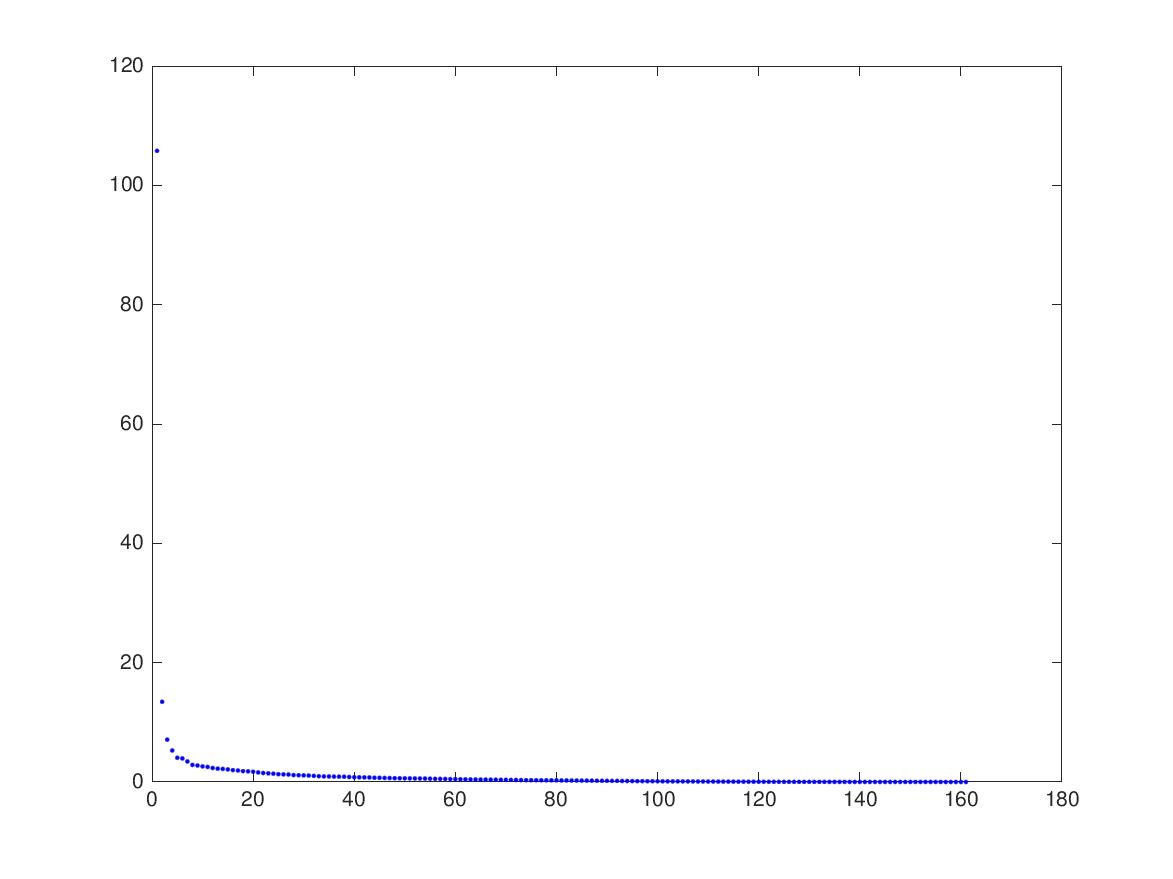
\includegraphics[width=0.7\linewidth]{SingularValues.jpg}
    \caption{Singular values}
    \end{figure}
    
\begin{solution}
    All the singular values are plotted in Fig. 2.
    As shown, the first singular value is very large ($>100$), while the following singular values are approximately between $[5, 20]$. When the index gets even larger, the singular values approaches zero (become very small).
    The condition number, which is 
    \begin{equation}
        cond(I)=\frac{\sigma_{max}}{\sigma_{min}}
    \end{equation}
    gets very large as a result. This suggests that it is ill-conditioned.

\end{solution}

\part
Let K=20, Extract the first K singular values and their corresponding vectors in U and V:

\begin{lstlisting}
K=20;
Sk=S(1:K,1:K);
Uk=U(:,1:K);
Vk=V(:,1:K);
\end{lstlisting}

Uk, Vk, Sk contain the compressed version of the image. To see this, form the compressed image:

\begin{lstlisting}
Imk=Uk*Sk*Vk';
imshow(Imk)
\end{lstlisting}

\textbf{Print out a copy of this compressed image and submit it.}
\begin{solution}
    The compressed image using the first 20 singular values is shown in Fig. 3 below.
\end{solution}

    \begin{figure}[!h]
    \centering
    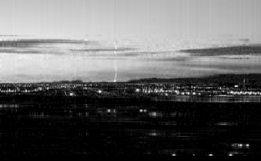
\includegraphics[width=0.7\linewidth]{k20_compressed001.png}
    \caption{Compressed image (K=20)}
    \end{figure}

\part
Repeat question (c) for K=40,60,80. \textbf{Submit the compressed images for the different values of K. Compare the 4 compressed images. Briefly describe what you notice.}
\begin{solution}
    The resultant images are shown in Fig. 4 - Fig. 6.
    As we take more singular values into computation (larger K), the quality of the compressed image improves. 
    \begin{equation}
        \Tilde{I} = s _ { 1 } u _ { 1 } v _ { 1 } ^ { T } + s _ { 2 } u _ { 2 } v _ { 2 } ^ { T } + \cdots + s _ { K } u _ { K } v _ { K } ^ { T }
    \end{equation}
    As shown in the equation above, larger K will give better approximation.

\end{solution}
    \begin{figure}[H]
    \centering
    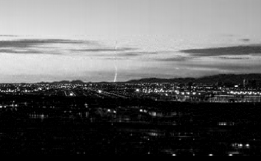
\includegraphics[width=0.6\linewidth]{k40_compressed001.png}
    \caption{Compressed image (K=40)}
    \end{figure}
    
    \begin{figure}[H]
    \centering
    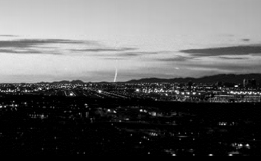
\includegraphics[width=0.6\linewidth]{k60_compressed001.png}
    \caption{Compressed image (K=60)}
    \end{figure}
    
    \begin{figure}[H]
    \centering
    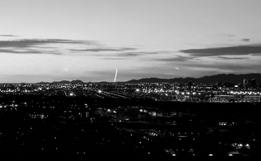
\includegraphics[width=0.6\linewidth]{k80_compressed001.png}
    \caption{Compressed image (K=80)}
    \end{figure}
\part
Thus, in image transmission, instead of transmitting the original image you can transmit $Uk, Vk, Sk$, which should be much less data than the original. \textbf{Is it worth transmitting when K=100} (i.e. do you save any bits in transmission when K=100)? Explain your answer.

\begin{solution}
    The total storage of the compressed image $I_{K}$ is expressed by:
    \begin{equation}
        S = K(m+n+1)
    \end{equation}
    For this question, $m=161, n=261$, so if we take $K=100$, the total storage we need for the transmission is $100 \times (161+261+1) = 42300$. This is even larger than the storage for just transmitting original image ($161 \times 261=42021$). Thus, transmitting compressed image with K=100 is \textbf{NOT} worth.
\end{solution}

\part
** Find an expression that bounds the per-pixel error (the difference between the original image and the compressed image for a particular pixel $(i, j)$) in terms of K, the singular values and the elements in U and V with the largest absolute magnitude $(u_{max}, v_{max}$ respectively).

\begin{solution}
    The completely re-constructed image (suppose $N$ non-zero singular values) and the compressed image using first K singular values are expressed by:
    \begin{equation}
        \begin{split}
            I 
            &= s _ { 1 } u _ { 1 } v _ { 1 } ^ { T } + s _ { 2 } u _ { 2 } v _ { 2 } ^ { T } + \cdots + s _ { K } u _ { K } v _ { K } ^ { T } + \cdots + s _ { n } u _ { n } v _ { n } ^ { T } \\
        \Tilde{I} 
        &= s _ { 1 } u _ { 1 } v _ { 1 } ^ { T } + s _ { 2 } u _ { 2 } v _ { 2 } ^ { T } + \cdots + s _ { K } u _ { K } v _ { K } ^ { T }
        \end{split}
    \end{equation}
    So the error term is their difference:
    \begin{equation}
        \varepsilon = |\sum_{n=K+1}^{N} s _ { n } u _ { n } v _ { n } ^ { T } |
    \end{equation}
    For a single pixel ($I_{i,j}$), the error is:
    \begin{equation}
        \begin{split}
        \epsilon 
        &= | \sum_{n=K+1}^{N} s _ { n } u _ { i, n } (v ^ { T })_{n, j} |\\
        &\leqslant \sum_{n=K+1}^{N} |s _ { n } u _ { i, n } (v ^ { T })_{n, j}|\\
        &\leqslant \sum_{n=K+1}^{N} s _ { n } |u _ { i, n }| |(v ^ { T })_{n, j}|\\
        &\leqslant \sum_{n=K+1}^{N} s _ { n } u _ { max } v _{max}\\
    \end{split}
    \end{equation}
    
\end{solution}

\part
** SVD is intimately related to PCA (Principal components analysis). Some of you might have learned about PCA in the EE3731C course, but it is not a pre-requisite for this question. Basically, finding the principal components of a matrix $X$ amounts to finding an orthonormal basis that spans the column space of $X$ (these are the column vectors $u_i$ in the matrix $U$). Here we create the data matrix $X$ by first vectorizing each of the 150 images into a column vector (by scanning in either row-major order or column- major order), and then stacking these vectors together into a matrix of size $42021\times150$. In effect, we have captured the entire video sequence into the 2D matrix $X$. \\\\
Before we proceed further, mean subtraction (a.k.a. "mean centering") to center the data at the origin is necessary for performing PCA. That is, the images are mean centered by subtracting the mean image vector from each image vector. This is to ensure that the first principal component $u_{1}$ really describes the direction of maximum variance. Again, if you do not have background in PCA, it is okay; just take it as a preprocessing step (or you can do some independent learning). \\\\
Apply SVD to the resultant mean-centered matrix. Take only the first $10$ principal components and reconstruct the image sequence. [NB: you can use the Matlab \mcode{reshape} command to convert a matrix to a vector and vice versa]. Observe the dynamics in the reconstructed video, comment on what you find, and explain why. Remember to add back this mean image vector when you are displaying your reconstructed results. \\\\
\text{[Non-mandatory]}: You can also explore other possibilities, like investigating what each principal component means, and their implications for processing and editing of outdoor webcam imagery.

\begin{solution}
    In principal component analysis we find the directions in the data with the most variation, i.e. the eigenvectors corresponding to the largest eigenvalues of the covariance matrix, and project the data onto these directions \cite{svd04}.
    
    Let's denote the elements in the data matrix $X$ as $X _ { j , \alpha } = x _ { j } ^ { \alpha }$. The mean vector is:
    \begin{equation}
        \langle \mathbf { x } \rangle \equiv \frac { 1 } { m } \sum _ { \alpha = 1 } ^ { m } \mathbf { x } ^ { \alpha }
    \end{equation}
    and the coariance matrix is:
    \begin{equation}
            C \equiv \frac { 1 } { m } \  X X  ^ { T },
    \end{equation}
    where we have removed the mean of the data: $X _ { j , \alpha } : = X _ { j , \alpha } - \left\langle x _ { j } \right\rangle$.
    
    Apply the SVD to $X$ and substitute $X$ in Eq. (11):
    \begin{equation}
        \begin{split}
            C &= \frac{1}{m} (U \Sigma V ^{T}) (U \Sigma V ^{T}) ^ {T}\\
            &= \frac{1}{m} U \Sigma V ^ {T} V \Sigma ^ {T} U ^ {T}\\
            &= \frac{1}{m} U \Sigma ^ {2} U ^ {T}
        \end{split}
    \end{equation}
    
    Clearly, the result in Eq. (12) demonstrates the Eigendecomposition of the real-valued symmetric matrix $mC$. Hence, the columns of $U$ are the eigenvectors of matrix $mC$ and the diagonal elements of $\Sigma ^ {2}$ are the eigenvalues. Therefore, the matrix $U$ after SVD of $X$ actually contains what we want for PCA. 
    
    Furthermore, if we denote the matrix of eigenvectors \textbf{sorted} according to eigenvalue by $\Tilde{U}$ , we can then use PCA to transform the data to be ${ Y } = \tilde {  U  } ^ { T }  { X }$. The eigenvectors are called the principal components. By selecting only the first $d$ rows of $Y$, we have projected the data from $n$ down to $d$ dimensions. \\\\
    In Matlab, to load all the images and construct the data matrix $X$, and do the mean subtraction:
    \begin{lstlisting}
X = [];
Files=dir('*.png');
for k=1:length(Files)
   FileNames=Files(k).name;
   I = im2double(imread(FileNames));
   I = I(:);
   X = [X I];
end
mean_X = mean(X, 2);
de_mean_X = X - mean_X;
    \end{lstlisting}
    Then, to calculate the SVD of matrix $X$ and transform the data into the first $10$ principle components' space:
    \begin{lstlisting}
[U S V] = svd(de_mean_X,0); % to produce "economy size"
X_PCAed = U(:,1:10) * S(1:10, :) * V';
X_reconstructed = X_PCAed + meanX;
for i=1:150
    Mat = X_reconstructed(:,i);
    Name = strcat('img_', int2str(i), '.png');
    imwrite(reshape(Mat, [161, 261]) ,Name,'png');
end
    \end{lstlisting}
    \textbf{Findings}\\
    By viewing the reconstructed video, I found that the only the light generated by planes sliding on the ground remains, while the light during the landing and taking off processes are nearly ``removed out". Besides, the light also gets blurry after PCA operation. This is because the operation only takes the first ten largest singular values out as valid information, and forms the orthogonal basis using these corresponding eigen-vectors. Every single image (column) is reconstructed using the principle components of all the images thus only the ``common" information remains; and between the frames (row) they are also ``smoothed out" thus things get blurry.
    
\end{solution}
\end{parts}
\end{questions}